\section{案例研究:SHA256}\label{sec:8-6}

NIST 于 1993 年发布了安全哈希算法(The Secure Hash Algorithm, SHA),作为数字签名标准 (Digital Signature Standard, DSS) 设计规范的一部分。这个哈希函数通常被称为 \textbf{SHA0},能够输出 $160$ 比特的摘要。两年之后的 1995 年,NIST 更新了该标准,在压缩函数中增加了一条额外的指令。由此产生的函数被称为 \textbf{SHA1}。NIST 并没有对这一修改作出解释,但是后来人们发现,这条额外的指令对抗碰撞来说至关重要。自此,SHA1 成为抗碰撞哈希的事实标准,并被广泛部署到各种系统中。

基于生日攻击,如果对该函数进行 $2^{80}$ 次计算,我们必然能够找到它的碰撞。2002 年,NIST 在 SHA 系列中增加了两个新的哈希函数:\textbf{SHA256} 和 \textbf{SHA512}。它们能输出更长的摘要(分别是 $256$ 和 $512$ 比特),因而能更好地防御生日攻击。NIST 还批准了 SHA224 和 SHA384,它们分别是将 SHA256 和 SHA512 的输出截断到 $224$ 和 $384$ 比特后得到的。表 \ref{tab:8-1} 总结了上述的哈希函数,并包含了其他的一些函数。

2004 到 2005 年是抗碰撞哈希函数的坏年头。一些新的攻击展示了高效地找到哈希碰撞的方法。特别是,王小云等人提出了一种针对 SHA1 的碰撞查找器,它只需要对该函数进行 $2^{63}$ 次计算,这远少于生日攻击所需的 $2^{80}$ 次。在使用了一种改进算法后,SHA1 的第一次碰撞于 2017 年被找到。因此,SHA1 不再被认为是抗碰撞的,因而不应该再被使用在实际的系统中。目前推荐的做法是使用 SHA256,我们将在下面介绍它。

\begin{table}
\centering
\begin{tabular}{l|ccccc}
\hline
\multicolumn{1}{c|}{\textbf{名称}} &
  \textbf{时间} &
  \textbf{\begin{tabular}[c]{@{}c@{}}摘要\\ 长度\end{tabular}} &
  \textbf{\begin{tabular}[c]{@{}c@{}}消息分组\\ 长度\end{tabular}} &
  \textbf{\begin{tabular}[c]{@{}c@{}}速度\footnotemark[2]\\ MB/秒\end{tabular}} &
  \textbf{\begin{tabular}[c]{@{}c@{}}已知最优\\ 攻击时间\end{tabular}} \\ \hline
SHA0     & 1993 & 160 & 512  &     & $2^{39}$ \\
SHA1     & 1995 & 160 & 512  & 153 & $2^{63}$ \\
SHA224   & 2004 & 224 & 512  &     &        \\
SHA256   & 2002 & 256 & 512  & 111 &        \\
SHA384   & 2002 & 384 & 1024 &     &        \\
SHA512   & 2002 & 512 & 1024 & 99  &        \\ \hline
MD4      & 1990 & 128 & 512  &     & $2^1$  \\
MD5      & 1992 & 128 & 512  & 255 & $2^{16}$ \\
Whirpool & 2000 & 512 & 512  & 57  &        \\ \hline
\end{tabular}
\caption{Merkle-Damg{\aa}rd 抗碰撞哈希函数}
\label{tab:8-1}
\end{table}

\footnotetext[2]{性能参数由 Wei Dai 提供,使用 Crypto++ 5.6.0 基准测试,在 1.83 GhZ 的 Intel Core 2 处理器上运行。数字越高越好。}

\begin{snote}[SHA256 函数。]
SHA256 是一个 Merkle-Damg{\aa}rd 哈希函数,它使用一个 Davies-Meyer 压缩函数 $h$。这个 $h$ 以一个 $256$ 比特的链式变量 $t$ 和一个 $512$ 比特的消息分组 $m$ 为输入,输出一个 $256$ 比特的链式变量。

我们首先描述 SHA256 的 Merkle-Damg{\aa}rd 链。回顾一下,在我们对 Merkle-Damg{\aa}rd 的介绍中,填充分组 $\mathrm{PB}$ 包含了对被哈希消息的\emph{分组}数量的 $64$ 比特编码。SHA256 与此大概相同,只是在 SHA256 中,$\mathrm{PB}$ 所编码的是被哈希消息的\emph{比特}数量,这一点略有不同。因此,SHA256 可以对最长 $2^{64}-1$ 比特的消息进行哈希。SHA256 中的 Merkle-Damg{\aa}rd 初始值 (IV) 被设定为下面的十六进制值:
\[
\mathrm{IV}:=\texttt{6a09e667 bb67ae85 3c6ef372 a54ff53a 510e527f 9b05688c 1f83d9ab 5be0cd19}\in\{0,1\}^{256}
\]

显然,为了获得更短的摘要,我们可以将 SHA256 的输出截短,但这是以牺牲安全性为代价的。事实上,这就是 SHA224 哈希函数的工作原理——除以下两点外,它与 SHA256 相同:(1) SHA224 使用另一个初始向量 IV,以及 (2) SHA224 将 SHA256 的输出截短,只保留最左边的 $224$ 比特。

接下来,我们介绍 SHA256 的 Davies-Meyer 压缩函数 $h$。它是由一个分组密码构建的,我们用 $E_\mathrm{SHA256}$ 表示。然而,SHA256 没有像 Davies-Meyer 中那样使用异或运算,而是使用模 $2^{32}$ 加法。也就是说,令:
\[
x_0,x_1,\dots,x_7\in\{0,1\}^{32},
\qquad
y_0,y_1,\dots,y_7\in\{0,1\}^{32}
\]
并设置:
\[
x:=x_0\,\Vert\,\cdots\,\Vert\,x_7\in\{0,1\}^{256},
\qquad
y:=y_0\,\Vert\,\cdots\,\Vert\,y_7\in\{0,1\}^{256}
\]
定义:
\[
x\boxplus y:=(x_0+y_0)\,\Vert\,\cdots\,\Vert\,(x_7+y_7)
\quad
\in\{0,1\}^{256}
\]
上面所有的加法都是模 $2^{32}$ 加法。那么,SHA256 的压缩函数 $h$ 的定义就是:
\[
h(t,m):=E_\mathrm{SHA256}(m,t)\boxplus t
\quad
\in\{0,1\}^{256}
\]
我们对 Davies-Meyer 的理想密码分析(定理 \ref{theo:8-4})同样适用于这个修改后的函数。
\end{snote}

\begin{snote}[SHA256 的分组密码。]
为了完成对 SHA256 的介绍,我们还需要描述分组密码 $E_\mathrm{SHA256}$。该算法使用了表 \ref{tab:8-2} 中定义的几个辅助函数。这里,SHR 和 ROTR 表示标准的右移和右旋函数。

\begin{table}
\centering
\begin{tabular}{rlll}
\multicolumn{4}{l}{对于 $x,y,z\in\{0,1\}^{32}$,定义:}                                                                 \\
\multicolumn{1}{l}{}   &    &                                                                              &      \\
$\mathrm{SHR}^{n}(x)$  & := & $(x>>n)$                                                                     & (左移) \\
$\mathrm{ROTR}^{n}(x)$ & := & $(x>>n)\lor(x<<32-n)$                                                        & (左旋) \\
\multicolumn{1}{l}{}   &    &                                                                              &      \\
$\mathrm{Ch}(x,y,z)$   & := & $(x\land y)\oplus(\lnot x\land z)$                                           &      \\
$\mathrm{Maj}(x,y,z)$  & := & $(x\land y)\oplus(x\land z)\oplus(y\land z)$                                 &      \\
\multicolumn{1}{l}{}   &    &                                                                              &      \\
$\Sigma_0(x)$          & := & $\mathrm{ROTR}^{2}(x)\oplus\mathrm{ROTR}^{13}(x)\oplus\mathrm{ROTR}^{22}(x)$ &      \\
$\Sigma_1(x)$          & := & $\mathrm{ROTR}^{6}(x)\oplus\mathrm{ROTR}^{11}(x)\oplus\mathrm{ROTR}^{25}(x)$ &      \\
$\sigma_0(x)$          & := & $\mathrm{ROTR}^{7}(x)\oplus\mathrm{ROTR}^{18}(x)\oplus\mathrm{SHR}^{3}(x)$   &      \\
$\sigma_1(x)$          & := & $\mathrm{ROTR}^{17}(x)\oplus\mathrm{ROTR}^{19}(x)\oplus\mathrm{SHR}^{10}(x)$ &     
\end{tabular}
\caption{SHA256分组密码中所使用的函数}
\label{tab:8-2}
\end{table}

密码 $E_\mathrm{SHA256}$ 接受一个 $512$ 比特的密钥 $k$ 和一条 $256$ 比特的消息 $t$ 作为输入。我们首先将密钥和消息拆分成 $32$ 比特长的字。我们记:
\[
\begin{aligned}
&k:=k_0\,\Vert\,k_1\,\Vert\,\cdots\,\Vert\,k_{15}\quad\in\{0,1\}^{512}\\
&t:=t_0\,\Vert\,t_1\,\Vert\,\cdots\,\Vert\,t_{7}\quad\in\{0,1\}^{256}
\end{aligned}
\]
其中,所有的 $k_i$ 和 $t_i$ 都在 $\{0,1\}^{32}$ 上。

表 \ref{tab:8-3} 展示了 $E_\mathrm{SHA256}$ 的伪代码。它将同一个轮函数迭代了 $64$ 次。该密码在每一轮中都会使用一个轮密钥 $W_i\in\{0,1\}^{32}$,这个轮密钥是在密钥设置步骤中被递归定义的。图 \ref{fig:8-8} 展示了该密码的其中一轮,它非常像两个相接的 Feistel 轮。该密码使用 $64$ 个固定的常数 $K_0,K_1,\dots,K_{63}\in\{0,1\}^{32}$,它们的值都被规定在了 SHA256 标准之中。比如说 $K_0:=\mathtt{428A2F98}$,$K_1:=\mathtt{71374491}$,都以十六进制表示。

\begin{table}
\hspace*{5pt} 输入:明文 $t:=t_0\,\Vert\,t_1\,\Vert\,\cdots\,\Vert\,t_{7}\in\{0,1\}^{256}$ 和密钥 $k:=k_0\,\Vert\,k_1\,\Vert\,\cdots\,\Vert\,k_{15}\in\{0,1\}^{512}$\\
\hspace*{5pt} 输出:$\{0,1\}^{256}$ 上的密文\\
\hspace*{20pt} // \emph{这里,所有的加法都是模 $2^{32}$ 加法}\\
\hspace*{20pt} // \emph{算法使用常数 $K_0,K_1,\dots,K_{63}\in\{0,1\}^{32}$ }

\vspace{15pt}

\hspace*{5pt} \underline{密钥设置}:构造 $64$ 个轮密钥 $W_0,\dots,W_{63}\in\{0,1\}^{32}$:

\vspace{5pt}

\hspace*{40pt}
\(
\left\{
\begin{array}{ll}
\text{对于}\;\, i=0,1,\dots,15, & \text{令}\;\, W_i\leftarrow k_i, \\
\text{对于}\;\, i=16,17,\dots,63, & \text{令}\;\, W_i\leftarrow \sigma_i(W_{i-2}) + W_{i-7} + \sigma_0(W_{i-15}) + W_{i-16}
\end{array}
\right.
\)

\vspace{15pt}

\hspace*{5pt} \underline{$64$ 轮加密}:

\vspace{5pt}

\hspace*{20pt} 令 $(a_0,b_0,c_0,d_0,e_0,f_0,g_0,h_0)\leftarrow(t_0,t_1,t_2,t_3,t_4,t_5,t_6,t_7)$\\
\hspace*{20pt} 对于 $i=0,\dots,63$:\\
\hspace*{45pt} 令 $T_1\leftarrow h_i+\Sigma_1(e_i)+\mathrm{Ch}(e_i,f_i,g_i)+K_i+W_i$\\
\hspace*{45pt} 令 $T_2\leftarrow \Sigma_0(a_i)+\mathrm{Maj}(a_i,b_i,c_i)$\\
\hspace*{45pt} 令 $(a_{i+1},b_{i+1},c_{i+1},d_{i+1},e_{i+1},f_{i+1},g_{i+1},h_{i+1})\leftarrow(T_1+T_2,a_i,b_i,c_i,d_i+T_1,e_i,f_i,g_i)$

\vspace{15pt}

\hspace*{5pt} \underline{输出}:$a_{64}\,\Vert\,b_{64}\,\Vert\,c_{64}\,\Vert\,d_{64}\,\Vert\,e_{64}\,\Vert\,f_{64}\,\Vert\,g_{64}\,\Vert\,h_{64}\in\{0,1\}^{256}$

\caption{SHA256分组密码}
\label{tab:8-3}
\end{table}

有趣的是,NIST 从来都没有给分组密码 $E_\mathrm{SHA256}$ 起一个正式的名字。该密码被 Handschuh 和 Naccache 命名为\textbf{SHACAL-2}。类似地,SHA1 的底层分组密码被称为 SHACAL-1。SHACAL-2 分组密码与我们上面介绍的 $E_\mathrm{SHA256}$ 基本相同,唯一的区别是,它可以使用短于 $512$ 比特的密钥进行加密。给定一个密钥 $k\in\{0,1\}^{\leq512}$,SHACAL-2 密码会将零缀在密钥后面来得到一个 $512$ 比特长的密钥。然后,它就将 $E_\mathrm{SHA256}$ 应用于给定的 $256$ 比特消息分组。SHACAL-2 的解密与加密类似。这个密码很适合已经实现了 SHA256 的应用,因为它能够有效减少代码库的整体规模。
\end{snote}

\begin{figure}
	\centering
	

\tikzset{every picture/.style={line width=0.75pt}} %set default line width to 0.75pt        

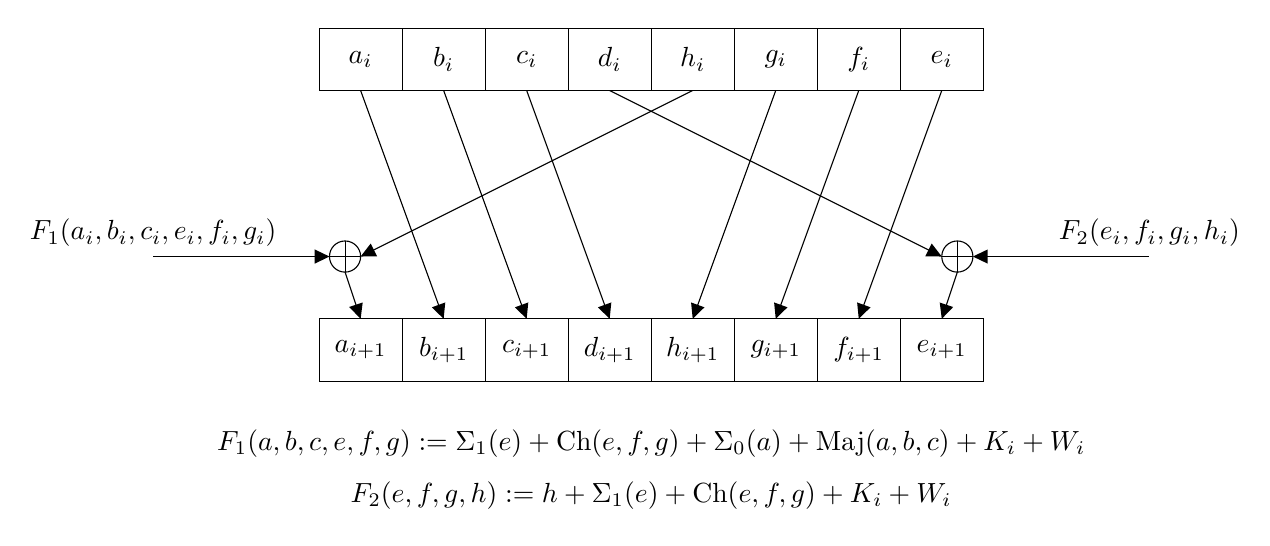
\begin{tikzpicture}[x=0.75pt,y=0.75pt,yscale=-1,xscale=1]
%uncomment if require: \path (0,253); %set diagram left start at 0, and has height of 253

%Shape: Rectangle [id:dp605201676603677] 
\draw   (100,0) -- (420,0) -- (420,30) -- (100,30) -- cycle ;
%Straight Lines [id:da7412689699456203] 
\draw    (140,0) -- (140,30) ;
%Straight Lines [id:da22647453790635086] 
\draw    (180,0) -- (180,30) ;
%Straight Lines [id:da8843056440098953] 
\draw    (220,0) -- (220,30) ;
%Straight Lines [id:da4329570184014415] 
\draw    (260,0) -- (260,30) ;
%Straight Lines [id:da4312753541741339] 
\draw    (300,0) -- (300,30) ;
%Straight Lines [id:da8624712063258593] 
\draw    (340,0) -- (340,30) ;
%Straight Lines [id:da48275098633745395] 
\draw    (380,0) -- (380,30) ;
%Shape: Rectangle [id:dp4067435943587554] 
\draw   (100,140) -- (420,140) -- (420,170) -- (100,170) -- cycle ;
%Straight Lines [id:da9101745062627391] 
\draw    (140,140) -- (140,170) ;
%Straight Lines [id:da6991884949951528] 
\draw    (180,140) -- (180,170) ;
%Straight Lines [id:da7121791754293847] 
\draw    (220,140) -- (220,170) ;
%Straight Lines [id:da006685736169755652] 
\draw    (260,140) -- (260,170) ;
%Straight Lines [id:da5006459019159044] 
\draw    (300,140) -- (300,170) ;
%Straight Lines [id:da2102106457102897] 
\draw    (340,140) -- (340,170) ;
%Straight Lines [id:da6413953387094566] 
\draw    (380,140) -- (380,170) ;
%Straight Lines [id:da9364234050345828] 
\draw    (120,30) -- (158.97,137.18) ;
\draw [shift={(160,140)}, rotate = 250.02] [fill={rgb, 255:red, 0; green, 0; blue, 0 }  ][line width=0.08]  [draw opacity=0] (7.14,-3.43) -- (0,0) -- (7.14,3.43) -- cycle    ;
%Straight Lines [id:da19670568284282752] 
\draw    (160,30) -- (198.97,137.18) ;
\draw [shift={(200,140)}, rotate = 250.02] [fill={rgb, 255:red, 0; green, 0; blue, 0 }  ][line width=0.08]  [draw opacity=0] (7.14,-3.43) -- (0,0) -- (7.14,3.43) -- cycle    ;
%Straight Lines [id:da9941673597047744] 
\draw    (200,30) -- (238.97,137.18) ;
\draw [shift={(240,140)}, rotate = 250.02] [fill={rgb, 255:red, 0; green, 0; blue, 0 }  ][line width=0.08]  [draw opacity=0] (7.14,-3.43) -- (0,0) -- (7.14,3.43) -- cycle    ;
%Straight Lines [id:da847071183150921] 
\draw    (320,30) -- (281.03,137.18) ;
\draw [shift={(280,140)}, rotate = 289.98] [fill={rgb, 255:red, 0; green, 0; blue, 0 }  ][line width=0.08]  [draw opacity=0] (7.14,-3.43) -- (0,0) -- (7.14,3.43) -- cycle    ;
%Straight Lines [id:da173533587645454] 
\draw    (360,30) -- (321.03,137.18) ;
\draw [shift={(320,140)}, rotate = 289.98] [fill={rgb, 255:red, 0; green, 0; blue, 0 }  ][line width=0.08]  [draw opacity=0] (7.14,-3.43) -- (0,0) -- (7.14,3.43) -- cycle    ;
%Straight Lines [id:da8735387545373061] 
\draw    (400,30) -- (361.03,137.18) ;
\draw [shift={(360,140)}, rotate = 289.98] [fill={rgb, 255:red, 0; green, 0; blue, 0 }  ][line width=0.08]  [draw opacity=0] (7.14,-3.43) -- (0,0) -- (7.14,3.43) -- cycle    ;
%Straight Lines [id:da32769861464522565] 
\draw    (240,30) -- (397.32,108.66) ;
\draw [shift={(400,110)}, rotate = 206.57] [fill={rgb, 255:red, 0; green, 0; blue, 0 }  ][line width=0.08]  [draw opacity=0] (7.14,-3.43) -- (0,0) -- (7.14,3.43) -- cycle    ;
%Straight Lines [id:da843529959376234] 
\draw    (280,30) -- (122.68,108.66) ;
\draw [shift={(120,110)}, rotate = 333.43] [fill={rgb, 255:red, 0; green, 0; blue, 0 }  ][line width=0.08]  [draw opacity=0] (7.14,-3.43) -- (0,0) -- (7.14,3.43) -- cycle    ;
%Flowchart: Or [id:dp6645760821949267] 
\draw   (105,110) .. controls (105,105.86) and (108.36,102.5) .. (112.5,102.5) .. controls (116.64,102.5) and (120,105.86) .. (120,110) .. controls (120,114.14) and (116.64,117.5) .. (112.5,117.5) .. controls (108.36,117.5) and (105,114.14) .. (105,110) -- cycle ; \draw   (105,110) -- (120,110) ; \draw   (112.5,102.5) -- (112.5,117.5) ;
%Straight Lines [id:da07315377917091626] 
\draw    (112.5,117.5) -- (119.05,137.15) ;
\draw [shift={(120,140)}, rotate = 251.57] [fill={rgb, 255:red, 0; green, 0; blue, 0 }  ][line width=0.08]  [draw opacity=0] (7.14,-3.43) -- (0,0) -- (7.14,3.43) -- cycle    ;
%Flowchart: Or [id:dp5992738702372278] 
\draw   (400,110) .. controls (400,105.86) and (403.36,102.5) .. (407.5,102.5) .. controls (411.64,102.5) and (415,105.86) .. (415,110) .. controls (415,114.14) and (411.64,117.5) .. (407.5,117.5) .. controls (403.36,117.5) and (400,114.14) .. (400,110) -- cycle ; \draw   (400,110) -- (415,110) ; \draw   (407.5,102.5) -- (407.5,117.5) ;
%Straight Lines [id:da3032162844879227] 
\draw    (407.5,117.5) -- (400.95,137.15) ;
\draw [shift={(400,140)}, rotate = 288.43] [fill={rgb, 255:red, 0; green, 0; blue, 0 }  ][line width=0.08]  [draw opacity=0] (7.14,-3.43) -- (0,0) -- (7.14,3.43) -- cycle    ;
%Straight Lines [id:da5583137617955998] 
\draw    (20,110) -- (102,110) ;
\draw [shift={(105,110)}, rotate = 180] [fill={rgb, 255:red, 0; green, 0; blue, 0 }  ][line width=0.08]  [draw opacity=0] (7.14,-3.43) -- (0,0) -- (7.14,3.43) -- cycle    ;
%Straight Lines [id:da3517569841519508] 
\draw    (418,110) -- (500,110) ;
\draw [shift={(415,110)}, rotate = 0] [fill={rgb, 255:red, 0; green, 0; blue, 0 }  ][line width=0.08]  [draw opacity=0] (7.14,-3.43) -- (0,0) -- (7.14,3.43) -- cycle    ;

% Text Node
\draw (20,106.6) node [anchor=south] [inner sep=0.75pt]    {$F_{1}( a_{i} ,b_{i} ,c_{i} ,e_{i} ,f_{i} ,g_{i})$};
% Text Node
\draw (500,106.6) node [anchor=south] [inner sep=0.75pt]    {$F_{2}( e_{i} ,f_{i} ,g_{i} ,h_{i})$};
% Text Node
\draw (120,15) node    {$a_{i}$};
% Text Node
\draw (160,15) node    {$b_{i}$};
% Text Node
\draw (200,15) node    {$c_{i}$};
% Text Node
\draw (240,15) node    {$d_{i}$};
% Text Node
\draw (280,15) node    {$h_{i}$};
% Text Node
\draw (320,15) node    {$g_{i}$};
% Text Node
\draw (360,15) node    {$f_{i}$};
% Text Node
\draw (400,15) node    {$e_{i}$};
% Text Node
\draw (120,155) node    {$a_{i+1}$};
% Text Node
\draw (160,155) node    {$b_{i+1}$};
% Text Node
\draw (200,155) node    {$c_{i+1}$};
% Text Node
\draw (240,155) node    {$d_{i+1}$};
% Text Node
\draw (280,155) node    {$h_{i+1}$};
% Text Node
\draw (320,155) node    {$g_{i+1}$};
% Text Node
\draw (360,155) node    {$f_{i+1}$};
% Text Node
\draw (400,155) node    {$e_{i+1}$};
% Text Node
\draw (260,200) node    {$F_{1}( a,b,c,e,f,g) :=\Sigma _{1}( e) +\mathrm{Ch}( e,f,g) +\Sigma _{0}( a) +\mathrm{Maj}( a,b,c) +K_{i} +W_{i}$};
% Text Node
\draw (260,225) node    {$F_{2}( e,f,g,h) :=h+\Sigma _{1}( e) +\mathrm{Ch}( e,f,g) +K_{i} +W_{i}$};


\end{tikzpicture}
	\caption{SHA256分组密码的一轮}
	\label{fig:8-8}
\end{figure}
 
\subsection{其他 Merkle-Damg{\aa}rd 哈希函数}\label{subsec:8-6-1}

\begin{snote}[MD4和MD5。]
这两个密码学哈希函数都是由 Ron Rivest 在1990 到 1991 年设计的。它们两者都是 Merkle-Damg{\aa}rd 哈希函数,输出 $128$ 比特的摘要。它们非常相似,尽管 MD5 使用了比 MD4 更强的压缩函数。如表 \ref{tab:8-1} 所示,已经有算法能够有效地找到这两个哈希函数的碰撞。因此,它们都不应该再被使用在现实世界的系统之中。
\end{snote}

\begin{snote}[Whirpool。]
Whirlpool 由 Barreto 和 Rijmen 在 2000 年设计,并在 2004 年被采纳为 ISO/IEC 标准。Whirpool 是一个 Merkle-Damg{\aa}rd 哈希函数。它的压缩函数使用 Miyaguchi-Preneel 方法(见图 \ref{fig:8-7})和一个名为 $W$ 的分组密码。这个分组密码与 AES 非常相似,但是分组长度为 $512$ 比特。由此产生的哈希输出也是 $512$ 比特。
\end{snote}

\begin{snote}[其他算法。]
还有一些文献提出了许多其他的 Merkle-Damg{\aa}rd 哈希函数,比如 Tiger/192 和 RIPEMD-160。
\end{snote}